\documentclass[./exercises.tex]{subfiles}
\begin{document}
\textit{\textbf{Tentamen 2021-10-09 } }\\

\begin{enumerate}
\item  Du har $1.00$ kg vatten, som har temperaturen $+25.0^o$C , i en termos.
     Hur mycket is, med temperaturen $0.00^o$C, måste du hälla i termosen
	 för att blandningens sluttemperatur ska bli $+10.0^o$C.
	 Isens smältentalpi är $334$ kJ/kg.\\

Givet
\begin{flalign*}
m_{H_20}&= 1.00\text{ kg}\\
T_{1,H_20} &=+25.0^o\text{C}\\
T_{is} &=0^o\text{C}\\
T_{2,H_20} &=+10.0^o\text{C}\\
c_H &=334 \text{ kJ/kg}\\
c &=4.18\text{ kJ/kg*K}\\
\rho_{is}&\approx \rho_{H_20}\approx  1000\text{kg/m}^3
\end{flalign*}
Sökt $m_{is}=m_2$\\

Massjämvikt
\begin{flalign*}
m_{H_20}+m_2 &=m_f\\
\end{flalign*}
Energi avgiven lika med energi upptagen
\begin{flalign*}
&m_{H_20}\cdot c\cdot(T_{2,H_20}-T_{1,H_20})\\
&\hspace{1em}\hspace{1em}+m_2\cdot c_H + m_2\cdot c\cdot (T_{2,H_20}-0)=0\\
\end{flalign*}

Obekanta är $m_f$ och $m_2$.
Sätter in $m_2 = m_f-m_{H_20}$.
\begin{flalign*}
&m_{H_20}\cdot c\cdot(T_{2,H_20}-T_{1,H_20})\\
&\hspace{1em}+(m_f-m_{H_20})\cdot c_H\\
&\hspace{2em}+ (m_f-m_{H_20})\cdot c\cdot (T_{2,H_20}-0)=0\\
\end{flalign*}

Samlar ihop termer av $m_{H_20}$ till vänster och termer
av $m_f$ till höger för att lösa ut $m_f$.
\begin{flalign*}
&m_{H_20}\cdot [c\cdot(T_{2,H_20}-T_{1,H_20} -T_{2,H_20})-c_H]\\
&=-m_f\cdot c_H -m_f\cdot c\cdot T_{2,H_20}\\
\end{flalign*}
Förkortar
\begin{flalign*}
&-m_{H_20}\cdot [c\cdot T_{1,H_20} +c_H]\\
&=-m_f\cdot (c_H +c\cdot T_{2,H_20})\\
\end{flalign*}
Förkortar
\begin{flalign*}
&m_{H_20}\cdot [c\cdot T_{1,H_20} +c_H]\\
&=m_f\cdot (c_H +c\cdot T_{2,H_20})\\
\end{flalign*}
Löser ut $m_f$
\begin{flalign*}
&m_{H_20}\cdot \frac{[c\cdot T_{1,H_20} +c_H]}{(c_H +c\cdot T_{2,H_20})}=m_f \\
\end{flalign*}
Sätter in siffror
\begin{flalign*}
m_f&=1.00\cdot \frac{[4180\cdot 25.0 +334000]}{(334000 +4180\cdot 10.0)}\\
   &=1.166844066
\end{flalign*}
Vilket betyder att den totala massa is som måste tillföras är
$1.166844066 -1.00 =0.16684$ kg, vilket med tre värdesiffror blir 167 gram. 

Jag hade inte behövt gå omvägen att även teckna massjämvikt. Gjorde detta tanklöst.
Det hade räckt att ställa upp energi jämvikt och lösa ut $m_{is}$

\begin{flalign*}
m_v\cdot c\cdot (25-10) &= m_i\cdot c_H + c\cdot m_i(10 -0)\iff\\
m_i &= \frac{m_v\cdot c\cdot (25-10)}{c_H+c\cdot 10}\\
    &=\frac{1.00\cdot 4180\cdot (25-10)}{334000+4180\cdot 10}\\
    &=0.166844066
\end{flalign*}

\vfill\null
\clearpage
\columnbreak
\newpage

\item I en trycktank finns $2m^3$ luft $(\kappa = 1.40)$, temperatur $+20^o$C 
och tryck 100 kPa. Med hjälp av en kompressor, som arbetar adiabatiskt,
ska trycket i tanken höjas 10 gånger.
Kompressorn suger in 20 liter luft, temperatur $+20^o$C  och tryck 100 kPa,
per sekund.
Hur länge måste kompressorn arbeta innan trycket i tanken har ökat 10 gånger?\\

Givet
\begin{flalign*}
V&=2\text{ m}^3\\
T&=20^o\text{C}\\
p_1 &= 100\text{kPa}\\
p_2 &= 10\cdot p_1\\
\dot{V} &=0.02 m^3/s\\
\kappa &= 1.4\\
\end{flalign*}
Sökt är $\Delta t$.

Massan $m_1$ i tanken innan kompressorn startar är
\begin{flalign*}
m_1 &=\frac{p_1\cdot V_1}{R\cdot T}
\end{flalign*}
Massa $m_2$ som måste finnas i tanken för att trycket ska bli $10\cdot p_1$ är
\begin{flalign*}
m_2 &=\frac{10\cdot p_1\cdot V_1}{R\cdot T}
\end{flalign*}

Den massa som kompressorn måste tillföra $m_{tillf}$ under tiden $\Delta t$
är således
\begin{flalign*}
m_{tillf}&=m_2-m_1\\
         &=\frac{10\cdot p_1\cdot V_1}{R\cdot T}-\frac{p_1\cdot V_1}{R\cdot T}\\
		 &=\frac{9\cdot p_1\cdot V_1}{R\cdot T}
\end{flalign*}

Massflödet per tidsenhet är
\begin{flalign*}
\dot{m}_{tillf}=\rho\cdot\dot{V} &=\frac{p_1}{R\cdot T}\cdot\dot{V}
\end{flalign*}

och tiden för att nå upp till $m_{tillf}$ är
\begin{flalign*}
\Delta t\cdot \dot{m}_{tillf}&=m_{tillf}\iff\\
           \Delta t &=\frac{m_{tillf}}{\dot{m}_{tillf}}  \\
                    &= \frac{\frac{9\cdot p_1\cdot V_1}{R\cdot T}}{\frac{p_1}{R\cdot T}\cdot\dot{V}}  \\  
					&=\frac{9\cdot V_1}{\dot{V}}\\
					&=\frac{9\cdot 2}{0.02}= 900s\\
\end{flalign*}
Svar tiden det tar, med en värdesiffra är 900 sekunder.
\textbf{Detta är fel svar! $m_2$ ska räknas ut med nytt $T_2$!}

\begin{flalign*}
\frac{T_2}{T_1}&=\Big(\frac{p_2}{p_1}\Big)^{\frac{\kappa -1}{\kappa}}\\
           T_2 &= T_1\cdot \Big(\frac{p_2}{p_1}\Big)^{\frac{\kappa -1}{\kappa}}\\
		       &=293\cdot \Big(\frac{10\cdot p_1}{p_1}\Big)^{\frac{1.4 -1}{1.4}}\\
			   &=565.694434563^o\text{C}\\
\end{flalign*}
Skillnaden i massa som kompressorn måste tillföra
\begin{flalign*}
m_{tillf}&=m_2-m_1\\
         &=\frac{10\cdot p_1\cdot V_1}{R\cdot T_2}-\frac{p_1\cdot V_1}{R\cdot T_1}\\
\end{flalign*}
Ny beräkning
\begin{flalign*}
\Delta t\cdot \dot{m}_{tillf}&=m_{tillf}\iff\\
           \Delta t &=\frac{m_{tillf}}{\dot{m}_{tillf}}  \\
                    &=\frac{\frac{10\cdot p_1\cdot V_1}{R\cdot T_2}-\frac{p_1\cdot V_1}{R\cdot T_1}}{\frac{p_1}{R\cdot T_1}\cdot\dot{V}}  \\
					&=\frac{\frac{10\cdot V_1}{T_2}-\frac{ V_1}{ T_1}}{\frac{1}{T_1}\cdot\dot{V}}  \\
					&=\frac{10\frac{T_1}{T_2}V_1-V_1}{\dot{V}} \\
                    &=\frac{10\frac{293}{565.69}2-2}{0.02} \\
					&=417.95 s\approx 418s
\end{flalign*}

\vfill\null
\clearpage
\columnbreak
\newpage

\item En behållare har volymen $15.0$ l och innehåller $1.00$ kg syrgas
$(\kappa = 1.40,  R= 260$ J/(kg$\cdot$K)), som har temperaturen $+27.0^o$C.
Gasen expanderar polytropiskt till slutvolymen $45.0$ l varvid trycket
blir $1.39$ MPa. Beräkna polytropexponenten.\\

Givet
\begin{flalign*}
V_1 &=0.015\text{ m}^3\\
m &=1.00\text{ kg}\\
T_1 &= +27^o\text{ C} = 300^o\text{ K}\\
V_2 &= 0.045\text{ m}^3\\
p_2 &=1.36\cdot 10^6\text{ Pa}
\end{flalign*}
Sökt är polytropexponenten $n$.
$p_1$ kan räknas ut
\begin{flalign*}
p_1 &= \frac{m\cdot R\cdot T_1}{V_1}\\
    &=\frac{1.00\cdot 260\cdot 300}{0.015}\\
    &=5.200000\cdot 10^6\text{ Pa}
\end{flalign*}
Polytrop processer förhåller sig såsom
\begin{flalign*}
p_1\cdot V_1^n &=p_2\cdot V_2^n\\
\end{flalign*}
Löser ut $n$
\begin{flalign*}
\frac{p_1}{p_2}  &=\frac{V_2^n}{V_1^n}\\
ln \frac{p_1}{p_2}&= n \cdot ln \frac{V_2}{V_1}\iff\\
n&= \frac{ln \frac{p_1}{p_2}}{ln \frac{V_2}{V_1}}\\
 &= \frac{ln \frac{5.2\cdot 10^6}{1.36\cdot 10^6}}{ln \frac{0.045}{0.015}}\\
 &=ln(5.2/1.36)/ln(3)=1.220789117\\
\end{flalign*}

Polytrop exponenten är (med tre värdesiffror) 1.22

\vfill\null
\clearpage
\columnbreak
\newpage

\item 10 liter torr luft med temperaturen $+20^o$C har trycket
$1.0$ bar = $100$ kPa. Luften genomgår en isokor tryckökning.
Trycket dubbleras. Behöver värme tillföras eller bortföras? Hur många Joule?
Hur mycket ändras luftens inre energi? 
Data för luft tas ur tabell sid 16 i formelsamlingen.\\

Eftersom volymen är konstant och det skall ske en fördubbling av trycket
så måste värme tullföras.

Givet
\begin{flalign*}
V_1 &=0.01 \text{ m}^3\\
T_1&=20^o\text{C}=293^o\text{K}\\
p_1 &=1 \text{ bar}=1\cdot 10^5\text{ Pa}\\
V_2 &=V_1\\
p_2 &=2\cdot p_1\\
\end{flalign*}

För isokora processer gäller
\begin{flalign*}
\frac{p_1}{T_1}&=\frac{p_2}{T_2}\\
\end{flalign*}
Löser ut $T_2$
\begin{flalign*}
T_2&=T_1\frac{p_2}{p_1}\\
   &=293\frac{2\cdotp_1}{p_1}\\
   &=586^o\text{K}
\end{flalign*}
Värmeenergin $Q_{12}$ som måste tillföras är
\begin{flalign*}
Q_{12}&=m\cdot\bar{c}_v\cdot(T_2-T_1)\\
\end{flalign*}
Vi behöver information om $m$ och $\hat{c}_v$.
Avseende $m$
\begin{flalign*}
m&=\frac{p_1\cdot V_1}{R\cdot T_1}\\
 &=\frac{1\cdot 10^5\cdot 0.01}{287\cdot 293}\\
 &=0.011891879
\end{flalign*}
Vi har data för $c_p$ på sidan 16 och väljer att
ta medelvärdet

\begin{flalign*}
\bar{c}_p &= \frac{c_p(20^o\text{C})+c_p(60^o\text{C})}{2}\\
          &=\frac{1009+1005}{2}\\
          &=1007          
\end{flalign*}
Relationen $R=c_p-c_v$ ger 
\begin{flalign*}
\bar{c}_v &={c}_p-R\\
          &=1007  -287  \\
          &= 720 \text{J/kg}\cdot\text{K}\\     
\end{flalign*}
Isättning nu i formeln för energin $Q_{12}$
\begin{flalign*}
Q_{12}&=m\cdot \bar{c}_v\cdot(T_2-T_1)\\
      &=0.011891879\cdot720\cdot(586-293)\\
      &=2508. 71079384\text{ J}
\end{flalign*}
Svar med två värdesiffror är att energin 2.5 kJ måste tillföras.

\vfill\null
\clearpage
\columnbreak
\newpage


\item Temperaturen i ett kylskåp ska vara $0.0^o$C, och rummet i vilket kylskåpet
är placerat har temperaturen $+20^o$C. Hur stort värmeläckage in i kylskåpet
kan vi tillåta om det drivs av en ideal carnotmaskin vars tillförda effekt
ligger på 10 watt.

Givet
\begin{flalign*}
T_1 &=+20^o\text{C}=293^o\text{K}\\
T_2 &= 0^o\text{C}=273^o\text{K}\\
\dot{W}_t &=10 \text{ W}\\
\end{flalign*}
Sökt $\dot{Q}_{tillf}$

\begin{figure}[h]
\centering
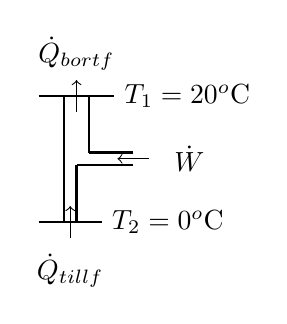
\begin{tikzpicture}[ scale=.4,baseline={(0,0)}]
%\draw upper 

\draw [thick] (1,0) -- (3,0) node[right]{    $T_2=0^o$C};%Basen för Q tillförd

\draw [thick] (1,4) -- (3.4,4) node[right]{    $T_1=20^o$C};%Basen för Q bortförd
\draw [thick] (1.8,0) -- (1.8,4); %Vänster kanalvägg
\draw [thick] (2.2,0) -- (2.2,1.8); %Höger kanalvägg
\draw [thick] (2.2,1.8)--(4,1.8); %w nedre kanalvägg
\draw [thick] (4,2.2)-- (2.6,2.2); %w övre kanalvägg
\draw [thick] (2.6,2.2)-- (2.6,4); %höger kanalvägg upp till bas

\draw[->] (2,-0.5) -- (2,0.5);
\node[below] (a) at (2,-0.7){$\dot{Q}_{tillf}$};

\draw[->] (4.5,2) -- (3.5,2);
\node[right] (b) at (5,2){$\dot{W}$};

\draw[->](2.2,3.5)--(2.2,4.5) node[above]{$\dot{Q}_{bortf}$};

\end{tikzpicture}
\end{figure}

Vi vet också att för Carnot kylmaskinen gäller
följande $T-s$-diagram
\begin{figure}[h]
\centering
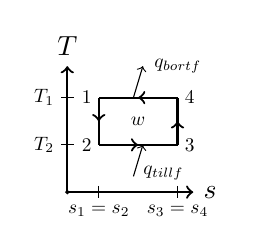
\begin{tikzpicture}[scale=.4,baseline={(0,0)}]
%\begin{tikzpicture}[show background rectangle, scale=.5]

%\draw (0,0) grid (4,4);
% x-axis
\draw [thick,->] (0,0) -- (4,0) node[right]{$s$};
% y-axis
\draw [thick,->] (0,0) -- (0,4) node[above]{$T$};
% x-axis label
%\node at (-0.3,4){$T$};
% y-axis label
%\node at (4,-0.3){$s$};
%origin point
\draw [color=black,fill=black] (0,0) circle (0.05);

\draw[thick](1,1.5)--(3.5,1.5)node[scale=0.7, right]{3};
\draw[thick,->](1,1.5)--(2.25,1.5);

\draw[thick](3.5,1.5)--(3.5,3)node[scale=0.7,right]{4};
\draw[thick,->](3.5,1.5)--(3.5,2.25);

\draw[thick](3.5,3)--(1,3)node[scale=0.7, left]{1};
\draw[thick,->](3.5,3)--(2.25,3);

\draw[thick](1,3)--(1,1.5)node[scale=0.7, left]{2};
\draw[thick,->](1,3)--(1,2.25);

\draw[->](2.1,0.5)--(2.4,1.5);%q_tillf pil
\draw[->](2.1,3)--(2.4,4);%q_bortf pil

\node[right,scale=0.7] (a) at (2.2,0.6){$q_{tillf}$};
\node[scale=0.7] (c) at (2.25,2.25){$w$};
\node[right,scale=0.7] (d) at (2.55,4.0){$q_{bortf}$};

\draw (1,0.2)--(1,-0.2) node[below,scale=0.7]{$s_1=s_2$};
\draw (3.5,0.2)--(3.5,-0.2) node[below,scale=0.7]{$s_3=s_4$};

\draw(0.2,3)--(-0.2,3) node[left,scale=0.7]{$T_1$};
\draw(0.2,1.5)--(-0.2,1.5) node[left,scale=0.7]{$T_2$};

\end{tikzpicture}
\end{figure}

Vi härleder köldfaktorn $\epsilon$ för en Carnot kylmaskin
\begin{flalign*}
\epsilon &=\frac{q_{tillf}}{w_t}\\
\epsilon_c &=\frac{T_2\cdot (s_3-s_2)}{T_1\cdot(s_3-s_2)-T_2\cdot(s_3-s_2)}\\
           &=\frac{T_2}{T-1-T_2}\\
           &=\frac{273}{293-273}\\
		   &=13.65\\
\end{flalign*} 
Kvoten $q_{tillf}/{w_t}$  är härledd under analys av en cykel men kvoten gäller också
över multipla cykler samt om man dividerar täljare och nämnare med tidsintervall $\Delta t$.\\
Således gäller framräknade $\epsilon$ även för kvoten
\begin{flalign*}
\epsilon &= \frac{\dot{Q}_{tillf}}{\dot{W}_t}\\       
\end{flalign*} 
Vi kan härifrån lösa ut det efterfrågae $\dot{Q}_{tillf}$
\begin{flalign*}
\dot{Q}_{tillf} &=\epsilon\cdot \dot{W}_t\\
                &=13.65\cdot 10
                &=136.5 W
\end{flalign*} 
Svar värmeläckaget (med en värdesiffra) får maximalt vara  136 W.

\vfill\null
\clearpage
\columnbreak
\newpage

\item  En ideal gas genomlöper följande kretsprocess medurs.\\
       -Uppvärmning vid konstant volym ifrån T1 till T2.\\
       -Adiabatisk expansion till T3.\\
       -Isoterm kompression tillbaks till startpunkten.\\
Rita ett pV-diagram och ett Ts-diagram över kretsprocessen. 
Beräkna processens termiska verkningsgrad om T1 är 200 K och T2 är 500 K.\\

Vi har 
\begin{flalign*}
&(1) \text{   isokor   } &(2)\\
&(2) \text{   adiabat  } &(3)\\
&(3) \text{   isoterm  } &(1)\\
\end{flalign*}
$q_{tillf}$ injiceras under isokoren och är
\begin{flalign*}
q_{tillf}&=c_v\cdot(T_2 - T_1)
\end{flalign*}
$q_{bortf}$ bortförs under isotermen och är
\begin{flalign*}
q_{bortf}&=R\cdot T_3\cdot ln\frac{v_4}{v_3}\\
         &=R\cdot T_1\cdot ln\frac{v_1}{v_3}&(1)\\
\end{flalign*}
eller
\begin{flalign*}
q_{bortf}&=R\cdot T_3\cdot ln\frac{p_3}{p_4}\\
         &=R\cdot T_1\cdot ln\frac{p_3}{p_1}&(2)\\
\end{flalign*}

Om vi antar att vi börjar vid tillståndet $(p_1,T_1,V_1)=(p_1,200^o\text{K},V_1)$
så går isokoren till tillståndet $(p_2,T_2,V_1)=(p_2,500^o\text{K},V_1)$
där
 \begin{flalign*}
\frac{p_1}{T_1}&=\frac{p_2}{T_2}\iff\\
p_2&=p_1\cdot \frac{T_2}{T_1}\\
    &=\frac{5}{2}\cdot p_1\\
\end{flalign*}
Då har vi\\
$(p_1,200^o\text{K},V_1)\underbrace{\rightarrow}_{isokor}(p_15/2,500^o\text{K},V_1)$\\
Därefter har vi adiabatiskt expansion
där 
\begin{flalign*}
p_2\cdot V_2^\kappa &=p_3\cdot V_3^\kappa\\
\end{flalign*}
eller 
\begin{flalign*}
\frac{T_3}{T_2}&=\Big(\frac{V_2}{V_3}\Big)^{\kappa-1}
\end{flalign*}
Men $T_3$ till $T_1$ är en isoterm så $T_3 =200^o\text{K}$.\\
\begin{flalign*}
\Big(\frac{T_3}{T_2}\Big)^{\frac{1}{\kappa -1}}&=\frac{V_2}{V_3}\iff\\
V_3&=\frac{V_2}{\Big(\frac{T_3}{T_2}\Big)^{\frac{1}{\kappa -1}}}\\
   &=\frac{V_1}{\Big(\frac{T_1}{T_2}\Big)^{\frac{1}{\kappa -1}}}\\
\end{flalign*}
Nu kan vi beräkna $q_{bortf}$
\begin{flalign*}
q_{bortf} &=R\cdot T_1\cdot ln\frac{v_1}{v_3}&(1)\\
      &=R\cdot T_1\cdot ln\frac{v_1}{\frac{v_1}{\Big(\frac{T_1}{T_2}\Big)^{\frac{1}{\kappa -1}}}}&(1)\\
	  &=R\cdot T_1\cdot ln \Big(\frac{T_1}{T_2}\Big)^{\frac{1}{\kappa -1}}\\
      &=R\frac{1}{\kappa -1}\cdot T_1\cdot ln \Big(\frac{T_1}{T_2}\Big)\\
\end{flalign*}

Nu kan vi beräkna verkningsgraden
\begin{flalign*}
\eta &= 1-\left|\frac{q_{bortf}}{q_{tillf}}\right|\\
&= 1-\left|\frac{R\frac{1}{\kappa -1}\cdot T_1\cdot ln \Big(\frac{T_1}{T_2}\Big)}{c_v\cdot(T_2 - T_1)}\right|\\
&= 1-\left|\frac{ T_1\cdot ln \Big(\frac{T_1}{T_2}\Big)}{(T_2 - T_1)}\right|\\
&=1-\left|\frac{ 200\cdot ln \Big(\frac{200}{500}\Big)}{(500 - 200)}\right|\\
&=0.389139512
\end{flalign*}
Verkningsgraden är $39\%$

Kunde ha beräknat detta mycket skonsammare om jag såsom läraren hade konstaterat
att $s_2-s_1$ är samma skillnad som $s_3-s_1$ och tagit $q_{bortf}$ såsom
$T_1\cdot (s_2-s_1)$
Vi beräknar $s_2-s_1$ för isokoren
\begin{flalign*}
s_2-s_1 &= \bar{c}_v\cdot ln\frac{T_2}{T_1}\\
\end{flalign*}
så 
\begin{flalign*}
\eta &= 1-\left|\frac{q_{bortf}}{q_{tillf}}\right|\\
       &= 1-\left|\frac{T_1\cdot\bar{c}_v\cdot ln\frac{T_2}{T_1}}{c_v\cdot(T_2 - T_1)}\right|\\
	   &= 1-\left|\frac{200\cdot\bar{c}_v\cdot ln\frac{500}{T_1}}{c_v\cdot(500 - 200)}\right|\\
\end{flalign*}
vilket ger samma resultat.

\vfill\null
\clearpage
\columnbreak
\newpage

\item Torr mättad vattenånga med trycket 20 bar expanderar
adiabatiskt ner till 5,0 bar då den passerar en turbin.
Beräkna hur mycket dess specifika volym ändras.\\

Adiabatisk expansion betyder att $s_1 = s_2$

$x_1=1$ läs av $s_1= s''$ för 20 bar.
Gå till bars raden och identfiera $x_2$ med $s_2 = s_1$
Räkna ut specifika volymen
\begin{flalign*}
v_2(5)&=(1-x_2)\cdot v' +x_2\cdot v''\\
\end{flalign*}
Specifika volymen har enheten kubikmeter per kg fuktig ånga.
Entalpin har enheten kJ per kg fuktig ånga.
Entropin har enheten kJ per kg fuktig ånga och Kelvin.

Formeln 
\begin{flalign*}
i_f &= t+x\cdot (2500+1.86\cdot t)
\end{flalign*}
har enheten kJ per kg torrluft. Dessa har jag blandatt ihop.

\item 1.0 kg luft med temperaturen +40 oC och $\varphi$=0.40 ska kylas ner till
+15 oC.  Hur mycket kondensat (vatten) måste bortföras för att inte dimma ska bildas?
Ta data ifrån bifogat Mollier-diagram.
Rita en förenklad skiss över Mollier-diagrammet där du markerar alla 
intressanta tillstånd och de värden du avläser i det bifogade Mollier-diagrammet.
Lämna in din skiss tillsammans med dina lösningar.\\

Ta fram vatteninnehållet (per kg torrluft), ta sedan fram max vatteninnehåll för 15 grader och $\varphi=1$
subtrahera mängderna.




\end{enumerate}

%\underbrace{}

% \hspace{1em}

%\begin{enumerate}[label=(\alph*)]
%\end{enumerate}


%\vfill\null
%\clearpage
%\columnbreak
%\newpage

%$$
%  A = 
%  \begin{bmatrix}
%    1 & 0  & 2i\\
%    2i & 0 &  -4\\
%    -i &  0 & -2i\\
%  \end{bmatrix}
%$$

%\begin{flalign*}
%  A = 
%  \begin{bmatrix}
%    1 & 0  & 2i\\
%    2i & 0 &  -4\\
%    -i &  0 & -2i\\
%  \end{bmatrix}
%\end{flalign*}


%\begin{flalign*}
%\psi(x) = \begin{cases} Ae^{ikx}+Be^{-ikx} &\ \  x<-a \\
%                        Ce^{\kappa x}+De^{-\kappa x} &\ \ -a < x < a\\
%						Fe^{ikx} & \ \ x>a
%       \end{cases}
%\end{flalign*}

%\begin{figure}[H]
%  \includegraphics[width=\linewidth]{odd_finite.eps}
%  \caption{$z_0=0.1\pi,0.5\pi, 3\pi,7\pi$}
%  \label{fig4}
%\end{figure}
\end{document}
